%Poster de MAC0215

\documentclass[final]{beamer}
\mode<presentation>{\usetheme{azul}}
\usepackage{graphicx}
\usepackage{epstopdf}
\usepackage{subfigure}

\usepackage[brazil]{babel}
\usepackage[utf8]{inputenc}
\usepackage{ragged2e}

\usepackage{mathtools}
\usepackage{amsmath,amsthm, amssymb, latexsym}
\usepackage[orientation=portrait,size=a2,scale=1.4]{beamerposter}
\usepackage[ruled]{algorithm2e}

\usepackage{enumerate}

\usepackage{snapshot} % will write a .dep file with all dependencies, allows for easy bundling

\DeclareMathSizes{17.42}{15}{14}{10}  % Math text size

%%%%%%%%%%%%%%%%%%%%%%%%%%%%%%%%
%%  MACROS %%%%%%%%%%%%%%%%%%%%%
\usepackage{xspace}
\newcommand{\pixel}{\emph{pixel}\xspace}
\newcommand{\pixels}{\emph{pixels}\xspace}
\newcommand{\voxel}{\emph{voxel}\xspace}
\newcommand{\voxels}{\emph{voxels}\xspace}

\newenvironment<>{spn-def}[1][\unskip]
  {\alert{\upshape\textbf{Definição #1}}
    \itshape}
  {\newline}

\newenvironment<>{spn-thm}[1][]
  {\alert{\upshape\textbf{Teorema}}
    \itshape}
  {\newline}

\listfiles
%%%%%%%%%%%%%%%%%%%%%%%%%%%%%%%%%%%%%%%%%%%%%%%%%%%%%%%%%%%%%%%%%%%%%%%%%%%%%%%%%%%%%%
\title{\huge Aprendizado Automático de Sum-Product Networks}

\author{Renato Lui Geh, Orientador: Denis Deratani Mauá}
\institute[Universidade de São Paulo] % (optional, but mostly needed)
{
  Instituto de Matemática e Estatística, Universidade de São Paulo - MAC0215 Atividade Curricular
  em Pesquisa
}

\date[Novembro 2015]{Novembro, 2015}
%%%%%%%%%%%%%%%%%%%%%%%%%%%%%%%%%%%%%%%%%%%%%%%%%%%%%%%%%%%%%%%%%%%%%%%%%%%%%%%%%%%%%%
\newlength{\columnheight}
\setlength{\columnheight}{65cm}
%%%%%%%%%%%%%%%%%%%%%%%%%%%%%%%%%%%%%%%%%%%%%%%%%%%%%%%%%%%%%%%%%%%%%%%%%%%%%%%%%%%%%%
\begin{document}
\begin{frame}
  \begin{columns}
    % ---------------------------------------------------------%
    % Set up a column
    \begin{column}{.5\textwidth}
      \begin{beamercolorbox}[center,wd=\textwidth]{postercolumn}
        \begin{minipage}[T]{1\textwidth} % tweaks the width, makes a new \textwidth
          \parbox[t][\columnheight]{\textwidth}{ % must be some better way to set the the height, width and textwidth simultaneously
            % Since all columns are the same length, it is all nice and tidy.  You have to get the height empirically
            % ---------------------------------------------------------%
            % fill each column with content
            \begin{block}{Motivação}
              \justifying
              Uma distribuição de probabilidades pode ser representada por uma função multilinear
              nas variáveis de uma distribuição com um número potencialmente exponencial de termos
              (ou seja, não compacta) como

              \begin{equation*}\tiny
                P(x_1,...,x_n) = \sum_\alpha c_\alpha \prod_{i \in \alpha} x_i\text{.}
              \end{equation*}

              O objetivo em Modelos Gráficos Probabilísticos (PGM) é computar inferência, ou seja,
              deseja-se encontrar a probabilidade

              \begin{equation*}\tiny
                P(x_q|x_{e_1},...,x_{e_m}) = \frac{P(x_qx_{e_1}...x_{e_m})}{P(x_{e_1}...x_{e_m})}
                \text{\small, onde $x_q$ é a query e $x_{e_1},...,x_{e_m}$ é a evidência.}
              \end{equation*}

              No entanto, inferência na maioria dos PGMs é intratável e, apesar de existirem
              modelos onde a inferência é, de fato, tratável, e serem representações compactas de
              distribuições, elas são limitadas em sua flexibilidade.\\~\\

              Em 2011\cite{poon-domingos}, Pedro Domingos e Hoifung Poon introduziram um novo tipo
              de modelo probabilístico que representa eficientemente uma função multilinear através
              de um digrafo acíclico enraizado (DAG), cuja inferência é sempre tratável e ainda
              assim é mais flexível que muitos outros modelos. Por meio de experimentos também
              comprovou-se que tanto inferência quanto aprendizado foram mais rápidos e precisos
              que outras redes profundas. \\~\\

              O objetivo desse estudo é aprender a definição, estrutura e propriedades de
              Sum-Product Networks e em seguida estudar os vários tipos de aprendizado que podemos
              efetuar neste modelo.

            \end{block}
            \vspace*{0.2cm}

            \begin{block}{Sum-Product Networks}
              \justifying
              Uma Sum-Product Network (SPN) tem definição recursiva. Seja $S$ uma SPN:
              \begin{itemize}
                \item Uma distribuição monovariável $P(X_i)$ é uma SPN.
                \item A soma $w_iS_i(X_\alpha)+w_jS_j(X_\beta)$ com pesos $w_j,w_i\geq0$ é uma SPN.
                  \hfill(1)
                \item O produto $S_i(X_\alpha) \cdot S_j(X_\beta)$ é uma SPN.\hfill(2)\\~\\
              \end{itemize}

              Podemos representar uma SPN com variáveis $x_1,...,x_d$ como um digrafo acíclico
              enraizado (DAG) cujas folhas são indicadores $x_1,...,x_d$ e $\overline{x}_1,...,
              \overline{x}_d$ e cujos nós internos são nós somas ou produtos. Toda aresta $ij$ onde
              $i$ tem origem em um nó soma tem um peso $w_{ij} \geq 0$ associado. O valor de um nó
              $i$ é $v_i$. O valor de um nó soma $i$ é $\sum_{j \in Ch(i)} w_{ij}v_j$. O valor de
              um nó produto $i$ é $\prod_{j \in Ch(i)} v_j$. $Ch(i)$ é o conjunto de nós filhos de
              $i$. O valor de um nó folha é o valor do indicador. O valor de uma SPN $S$ é o valor
              de sua raíz.

              \begin{figure}[h]
                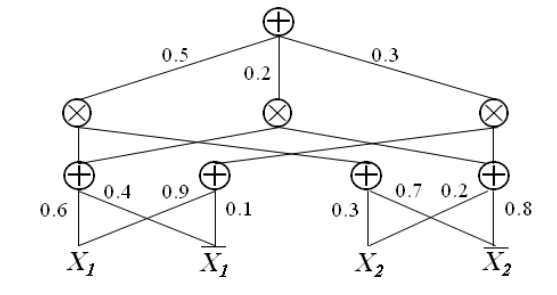
\includegraphics[scale=0.3]{spn_1.png}
                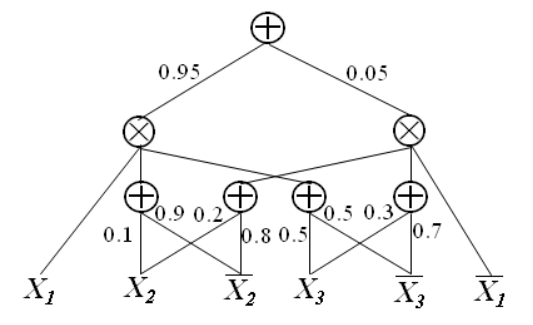
\includegraphics[scale=0.3]{spn_2.png}
                \caption{A esquerda uma SPN implementando uma naive Bayes mixture model. A direita
                  uma SPN implementando uma junction tree. Fonte: Poon e
                  Domingos\cite{poon-domingos}.}
              \end{figure}

              \begin{spn-def} Uma SPN $S$ é válida sse $\exists P:S(x)=P(x), \forall x$.
              \end{spn-def}
              \begin{spn-def} Uma SPN $S$ é completa sse $\alpha=\beta$ em (1).
              \end{spn-def}
              \begin{spn-def} Uma SPN $S$ é consistente sse $\alpha\cap\beta=\emptyset$ em (2).
              \end{spn-def}
              \begin{spn-thm} Uma SPN $S$ é válida se $S$ é completa e consistente.
              \end{spn-thm}

              SPNs válidas são desejáveis pois computam $P(x_1,...,x_n)$ em tempo linear em seu
              tamanho, além de completude e consistência permitirem que a inferência da SPN seja
              garantidamente eficiente.
            \end{block}
\vspace*{0.2cm}
            \begin{block}{Aprendizado}
                \justifying
                Pode-se dividir aprendizado de SPNs em duas classes:
                \begin{description}
                  \item[1] A partir de um DAG da SPN pré-definido, aprendemos os pesos do digrafo.
                  \item[2] Ambos DAG e pesos são desconhecidos e são aprendidos.\\~\\
                \end{description}

                O algoritmo proposto em \cite{poon-domingos} segue a primeira classe e é mostrado
                na seção seguinte. A partir de uma SPN densa e válida podemos aprender os pesos por
                Gradient Descent ou Expectation-Maximization (EM). \\~\\

                Gens e Domingos\cite{gens-domingos} propõem um outro método de aprendizado que
                explora a expressividade da SPN aprendendo-se não só os pesos como o próprio DAG.
                Para aprender o digrafo pode-se maximizar o estimador de semelhança $\max_S P(X^1,
                ...,X^N|S)$, onde $X^1,...,X^N$ são os conjuntos de dados.
           \end{block}
          }
        \end{minipage}
      \end{beamercolorbox}
    \end{column}
    % ---------------------------------------------------------%
    % end the column

    % ---------------------------------------------------------%
    % Set up a column
    \begin{column}{.5\textwidth}
      \begin{beamercolorbox}[center,wd=\textwidth]{postercolumn}
        \begin{minipage}[T]{1\textwidth} % tweaks the width, makes a new \textwidth
          \parbox[t][\columnheight]{\textwidth}{ % must be some better way to set the the height, width and textwidth simultaneously
            % Since all columns are the same length, it is all nice and tidy.  You have to get the height empirically
            % ---------------------------------------------------------%
            % fill each column with content

            \begin{block}{Algoritmo de Aprendizado de Pesos}

              \begin{algorithm}[H]
                \NoCaptionOfAlgo
                \KwIn{Conjunto $D$ de instâncias sobre variáveis $X$.}
                \KwOut{Uma SPN com estrutura e parâmetros construídos por aprendizado.}
                \tcc{Cria uma SPN inicial que seja válida.}
                $S \leftarrow$ GenerateDenseSPN($X$)\;
                InitializeWeights($S$)\;
                \Repeat{convergência}{
                  \ForAll{$d \in D$}{
                    \tcc{Atualiza pesos por Gradient Descent ou EM.}
                    UpdateWeights($S$, Inference($S$, $d$))\;
                  }
                }
                \tcc{Apara arestas com peso $w_{ij}=0$ e nós não-raíz sem pais.}
                $S \leftarrow$ PruneZeroWeights($S$)\;
                \KwRet{$S$}
              \end{algorithm}
            \end{block}
\vspace*{0.2cm}
            \begin{block}{Experimentos}
            \justifying
              Os experimentos mostrados a seguir foram extraídos a partir da implementação do
              algoritmo mostrado na seção anterior e mostram os resultados do código
              \cite{website:poon-domingos-code} implementado por Domingos e Poon e citados em
              \cite{poon-domingos}.

              \begin{figure}[h]
                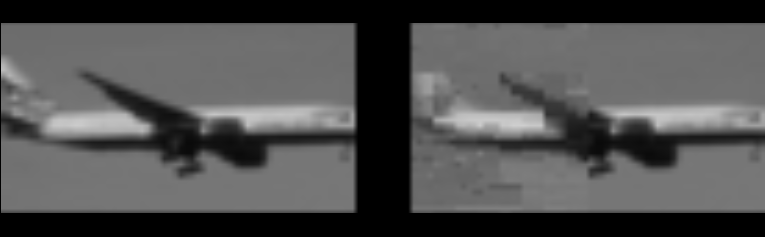
\includegraphics[scale=0.37025]{completions/plane0.png}
                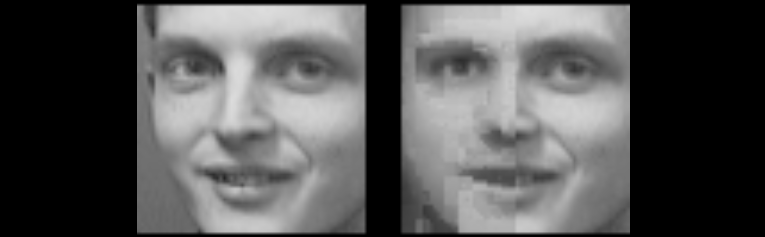
\includegraphics[scale=0.37025]{completions/face0.png} \\
                
\includegraphics[scale=0.37025]{completions/stop0.png}
                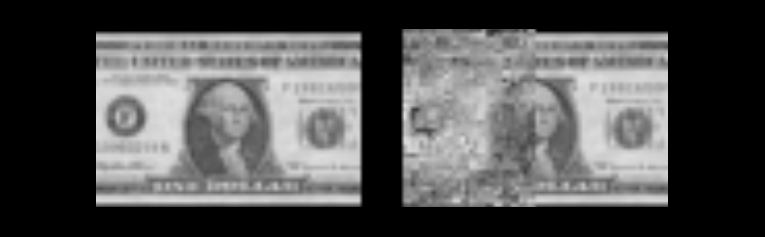
\includegraphics[scale=0.37025]{completions/dollar0.png}
                \caption{A saída do algoritmo consiste na compleção do lado esquerdo das imagens
                  a partir de um conjunto de treino. Para cada par de imagens, a imagem da esquerda
                  é a original, enquanto que a direita tem a metade esquerda completada pela SPN
                  e a outra metade igual a da original como evidência.}
              \end{figure}

              \begin{table}[h]
                \begin{center}
                  \begin{tabular}{l | r | r | r}
                    Arquitetura & Rostos & Motos & Carros \\
                    \hline
                    SPN & 99\% & 99\% & 98\% \\
                    CDBN & 95\% & 81\% & 87\% \\
                  \end{tabular}
                \end{center}
                \caption{\justifying Taxa média de acertos em uma comparação entre SPNs e CDBNs
                  (Convolutional Deep Belief Networks) em classificação (reconhecimento) de
                  imagens. SPNs obtiveram resultados quase perfeitos em reconhecimento.}
              \end{table}

              Pode-se ver que os resultados das SPNs são muito promissores e, dado que o algoritmo
              produzido por Domingos e Poon não toma muita vantagem da expressividade da estrutura
              local de SPNs, é fácil notar que ainda há muito espaço para melhorias.

            \end{block}
\vspace*{0.2cm}
            \begin{block}{Trabalhos futuros}
              \justifying
                Pretende-se estudar a implementação do método de aprendizado proposto por Poon e
                Domingos\cite{poon-domingos}, realizar outros experimentos com este algoritmo e
                explorar mais a fundo as propriedades de uma SPN.\\~\\

                Em seguida planeja-se estudar outros tipos de aprendizado em SPNs, principalmente
                métodos que estejam contidos na classe 2 de aprendizado e portanto tomem vantagem
                da estrutura local de SPNs, como o introduzido por Gens e
                Domingos\cite{gens-domingos}, buscas gulosas e clustering por Dennis e
                Ventura\cite{clustering, greedy-search} e Non-Parametric Bayesian Sum-Product
                Networks\cite{non-parametric-bayesian}.
                \vspace*{0.125cm}
            \end{block}
\vspace*{0.2cm}
            \begin{block}{Referências}
            \scriptsize
            \bibliographystyle{alpha}
            \bibliography{references}
\vspace*{0.22cm}
            \end{block}
            \vfill
          }
        \end{minipage}
      \end{beamercolorbox}
    \end{column}
    % ---------------------------------------------------------%
    % end the column


  \end{columns}
\end{frame}


\end{document}


%%%%%%%%%%%%%%%%%%%%%%%%%%%%%%%%%%%%%%%%%%%%%%%%%%%%%%%%%%%%%%%%%%%%%%%%%%%%%%%%%%%%%%%%%%%%%%%%%%%%
%%% Local Variables:
%%% mode: latex
%%% TeX-PDF-mode: t
%%% End:
